\subsection{Solceller}

En halvleder med et p-dopet og et n-dopet omr�de som ligger inntil hverandre kalles en pn-overgang. En slik pn-overgang har likerettende egenskaper. Det vil si at den leder str�m vesentlig bedre i den ene retningen enn den andre. Denne oppf�rselen definerer en diode. Siden p-siden har en konsentrasjon av elektroner i ledningsb�ndet som er vesentlig lavere enn n-sidens konsentrasjon av elektroner i ledningsb�ndet, vil vi f� en transport av ledningsb�nd-elektroner fra n-siden til p-siden ved diffusjon. Det samme skjer ogs� for hull fra p-siden til n-siden. Denne str�mmen av ladnings kalles diffusjonsstr�mmen. I prinsippet kan ogs� dopantene Si, B og P diffundere mellom de to delene av krystallen, men er bare betydelig for veldig h�ye temperaturer, alts� ikke vesentlig i romtemperatur.

Deplesjonssjiktet er et omr�de n�r grenseflaten mellom de to dopekonsentrasjonene som vil v�re essensielt t�mt for frie ladningsb�rere. Siden n-siden av deplesjonssjiktet inneholder donorer uten tilh�rende elektron vil denne siden v�re positivt ladet, og tilsvarende vil p-siden v�re negativt ladet. Dette gj�r at det oppst�r et elektrisk felt fra n- til p-siden, eller et fall i potensial fra n-siden til p-siden. Dette feltet f�rer til en driftstr�m som g�r i motsatt retning av diffusjonsstr�mmen og f�rer til 0 netto str�m, eller likevekt.

% figur fra s. 14 i kompendiet

\begin{figure}[!h]%

\begin{tikzpicture}

	\tikzstyle{box} 	=	[rectangle, draw, thick, fill=black!10, minimum width=15em, minimum height=3cm]
	\tikzstyle{ladning} 	=	[circle, draw, fill=black!20, minimum size=0.6cm]
	\def\edistance{0.6cm}
	
	\node[box]	(p)	{p};
	\node[box]	(n) [right of=p, node distance=15em]	{n};
	
	\node[ladning] (p3) [right of=p, node distance=8.35em] 	{\tiny{+}};
	\node[ladning] (p2) [above of=p3, node distance=\edistance] {\tiny{+}};
	\node[ladning] (p1) [above of=p2, node distance=\edistance] {\tiny{+}};
	\node[ladning] (p4) [below of=p3, node distance=\edistance] {\tiny{+}};
	\node[ladning] (p5) [below of=p4, node distance=\edistance] {\tiny{+}};
	
	\node[ladning] (n3) [left of=n, node distance=8.35em] 			{\small{-}};
	\node[ladning] (n2) [above of=n3, node distance=\edistance] {\small{-}};
	\node[ladning] (n1) [above of=n2, node distance=\edistance] {\small{-}};
	\node[ladning] (n4) [below of=n3, node distance=\edistance] {\small{-}};
	\node[ladning] (n5) [below of=n4, node distance=\edistance] {\small{-}};
	
	% Draw curly braces using path decoration
	\draw [thick,decorate,decoration={brace,amplitude=5pt}]
   (2.2,1.6) -- (3.5,1.6)
   node [black,midway,above=2pt] {\footnotesize $|E|>>0$};

	\draw [thick,decorate,decoration={brace,amplitude=5pt}]
   (-2.8,1.6) -- (2.1,1.6)
   node [black,midway,above=2pt] {\footnotesize N�ytralt, $E=0$};

	\draw [thick,decorate,decoration={brace,amplitude=5pt}]
   (3.6,1.6) -- (8.5,1.6)
   node [black,midway,above=2pt] {\footnotesize N�ytralt, $E=0$};

	% Str�mpiler
	\draw [thick,<-] (2,-1.8) -- (3.6,-1.8) node [right=2pt]	{$I_{drift}$}; 
	\draw [thick,->] (2,-2.3) -- (3.6,-2.3) node [left=45pt]	{$I_{diffusjon}$}; 

\end{tikzpicture}

\caption{Deplesjonssjiktet}%
\label{fig:deplesjonssjiktet}%
\end{figure}

Ved belysning genereres det minoritetsb�rere i pn-overgangen utover de som genereres termisk ved at fotoner eksiterer elektroner til ledningsb�ndet. Denne genereringen er ofte vesentlig st�rre enn driftstr�mmen. Denne str�mmen er uavhengig av potensialforskjellene i pn-overgangen. For en diode i m�rke er det gitt en str�m-spenning karakteristikk gitt av:

\begin{equation}
I=|I_{drift}|e^{\frac{qV}{kT}-1}
\label{eq:diodeiv}
\end{equation}

N�r pn-overgangen blir belyst vil driftstr�mmen �ke, og forskyve str�m-spenning karakteristikken nedover

% figur fra side 22 i kompendiet
\begin{figure}[!h]
\centering
\begin{tikzpicture}

	\draw [->] (-3,0) -- (3,0) node [right=5pt]	{V};  % Y-akse
	\draw [->] (0,-2) -- (0,3) node [above=5pt]	{I}; % X-akse

	% Diode
	\draw [dashed,-] (-3,-0.2) -- (-1,-0.2);
	\draw [dashed,-] (-1,-0.2) .. controls +(right:1.2cm) .. (1.5,3);
	\draw [->, >=triangle 45] (-2.5,0.5) -- node[right] {$I_{drift}$} (-2.5,0);
	\draw [->, >=triangle 45] (-2.5,-0.7) -- (-2.5,-0.2);
	
	% Solcelle
	\draw [-] (-3,-1.8) -- (-1,-1.8);
	\draw [-] (-1,-1.8) .. controls +(right:1.5cm) .. (1.5,2);
	\draw [<->, >=triangle 45] (-1.7,-1.8) -- node[right] {$I_{belysning}$} (-1.7,-0.2);

\end{tikzpicture}

\caption{Str�m-spenningskarakterisitikken for en solcelle}%
\label{fig:ivsolcelle}%
\end{figure}

For solceller defineres ofte str�m ut av cellen som positiv, slik at karakteristikken vendes om V-aksen

\begin{equation}
I=I_{belysning}-I_{drift}(e^{\frac{qV}{kT}-1})
\label{eq:solcelleiv}
\end{equation}

hvor $I_{belysning}$ er str�m generert av lys. Spenningen ved �pen krets er gitt ved:

\begin{equation}
V_{OC}=\frac{kT}{q}\ln(\frac{I_{belysning}}{I_{drift}}+1)
\label{eq:voc}
\end{equation}

Maks effekt som genereres av solcellen er gitt av:

\begin{equation}
P_m=I_m V_m
\label{eq:piv}
\end{equation}

Hvor $P_m$ er maks effekt, $I_m$ er maks str�m og $V_m$ er maks spenning. Fyllfaktoren FF er gitt av faktisk effekt ut, over teoretisk maks effekt:

\begin{equation}
FF=\frac{I_m V_m}{I_{belysning} V_{OC}}
\label{eq:fyllfaktor}
\end{equation}

hvor $V_{OC}$ er spenning ved �pen krets.

% fyllfaktor figur
\begin{figure}[!h]
\centering
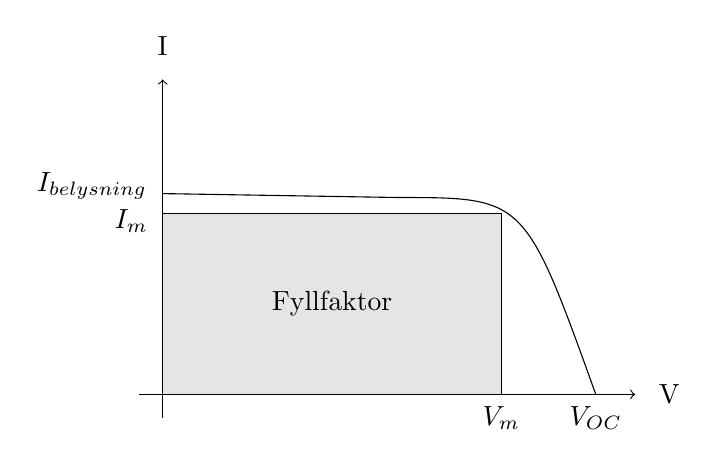
\begin{tikzpicture}

	\draw [->] (-0.3,0) -- (6,0) node [right=5pt]	{V};  % X-akse
	\draw [->] (0,-0.3) -- (0,4) node [above=5pt]	{I}; % Y-akse

	% Faktisk kurve
	\draw [-] (0,2.55) -- (3,2.5);
	\draw [-] (3,2.5) .. controls +(right:1.6cm) .. (5.5,0);
	
	% Fyllfaktor
	\node [draw, rectangle,fill=black!10,minimum height=2.3cm, minimum width=4.3cm] (FF) at (2.15,1.15) {Fyllfaktor};
	
	% Tekst
	\node at (-0.9,2.65) {$I_{belysning}$};
	\node at (-0.4,2.2) {$I_m$};
	\node at (4.3,-0.3) {$V_m$};
	\node at (5.5,-0.3) {$V_{OC}$};
	
	
\end{tikzpicture}

\caption{Str�m-spenningskarakterisitikken for en solcelle}%
\label{fig:fyllfaktor}%
\end{figure}

Virkningsgraden til en solcelle er representert ved $\eta$, som er gitt ved:

\begin{equation}
\eta=\frac{P_m}{P_{inn}}=FF \frac{I_{belysning} V_{OC}}{P_{inn}}
\label{eq:virkningsgrad}
\end{equation}
